\documentclass{beamer}
\usepackage{relsize}
\usepackage{color}

\usepackage{listings}
\usetheme{CambridgeUS}
%\usepackage{beamerthemesplit} % new 
\usepackage{enumitem}
\usepackage{amsmath}                    % See geometry.pdf to learn the layout options. 
\usepackage{amsthm}                   % See geometry.pdf to learn the layout options. There 
\usepackage{amssymb}                    % See geometry.pdf to learn the layout options. 
\usepackage[utf8]{inputenc} 
\usepackage{graphicx}
\usepackage[english,bulgarian]{babel}

\lstset{language=C++,
                basicstyle=\ttfamily,
                keywordstyle=\color{blue}\ttfamily,
                stringstyle=\color{red}\ttfamily,
                commentstyle=\color{green}\ttfamily,
                morecomment=[l][\color{magenta}]{\#}
}

\newtheorem{mydef}{Дефиниция}[section]
\newtheorem{lem}{Лема}[section]
\newtheorem{thm}{Твърдение}[section]

\DeclareMathOperator{\restrict}{\upharpoonright}

\setitemize{label=\usebeamerfont*{itemize item}%
  \usebeamercolor[fg]{itemize item}
  \usebeamertemplate{itemize item}}

\setbeamercovered{transparent}



\begin{document}
\title[Обектно ориентирано програмиране]{Жизнен цикъл на обектите. Конструктори} 
\author{Калин Георгиев} 
\frame{\titlepage} 

\section{Динамична памет} 


\begin{frame}
\centerline{Жизнен цикъл на обектите (променливите)}
\end{frame}


\begin{frame}[fragile]
\frametitle{Локална променлива}
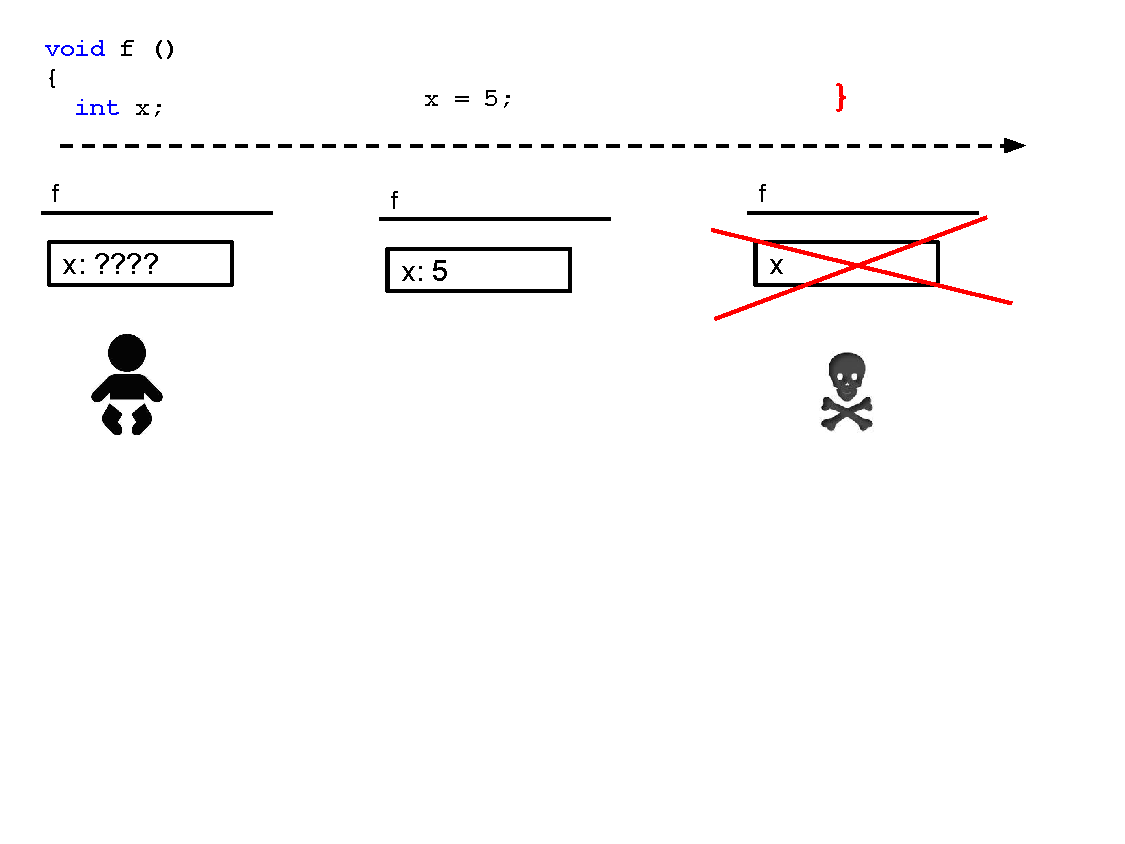
\includegraphics[width=12.5cm]{images/lc_var}
\end{frame}


\begin{frame}[fragile]
\frametitle{Параметър}
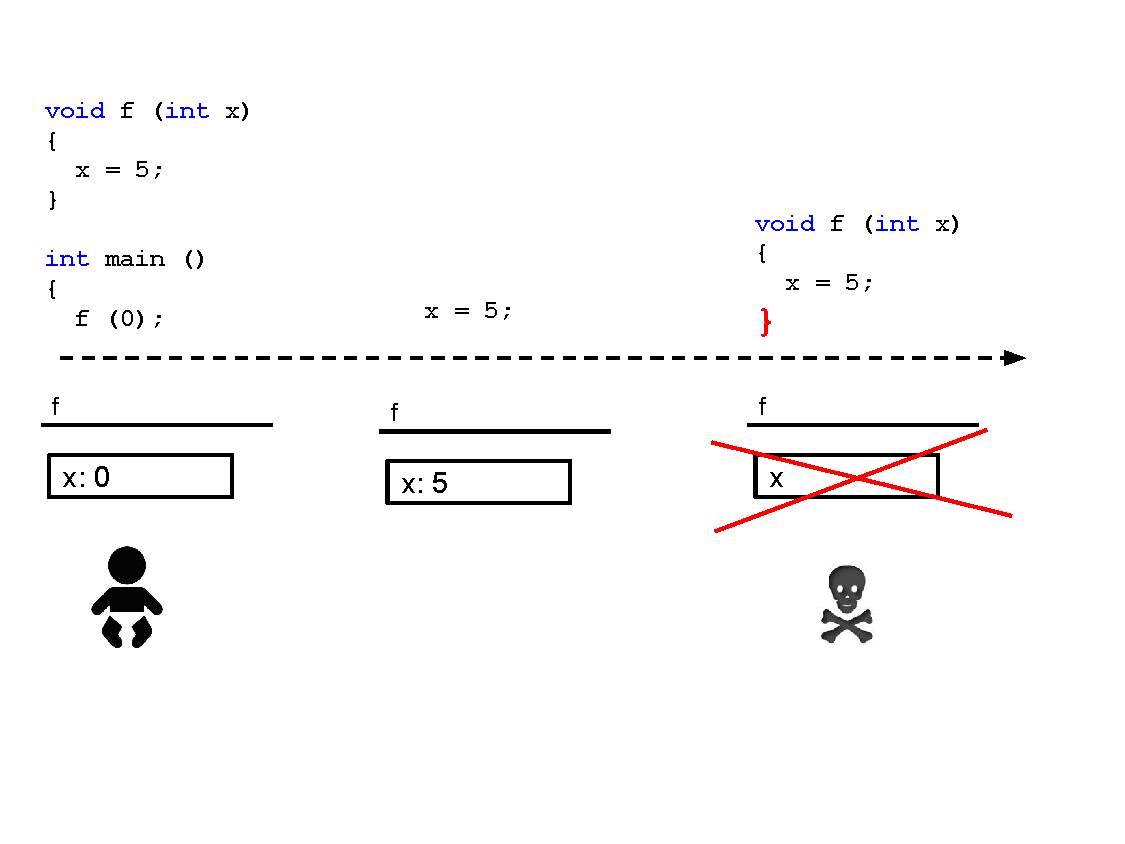
\includegraphics[width=12.5cm]{images/lc_par}
\end{frame}

\begin{frame}[fragile]
\frametitle{Динамична памет}
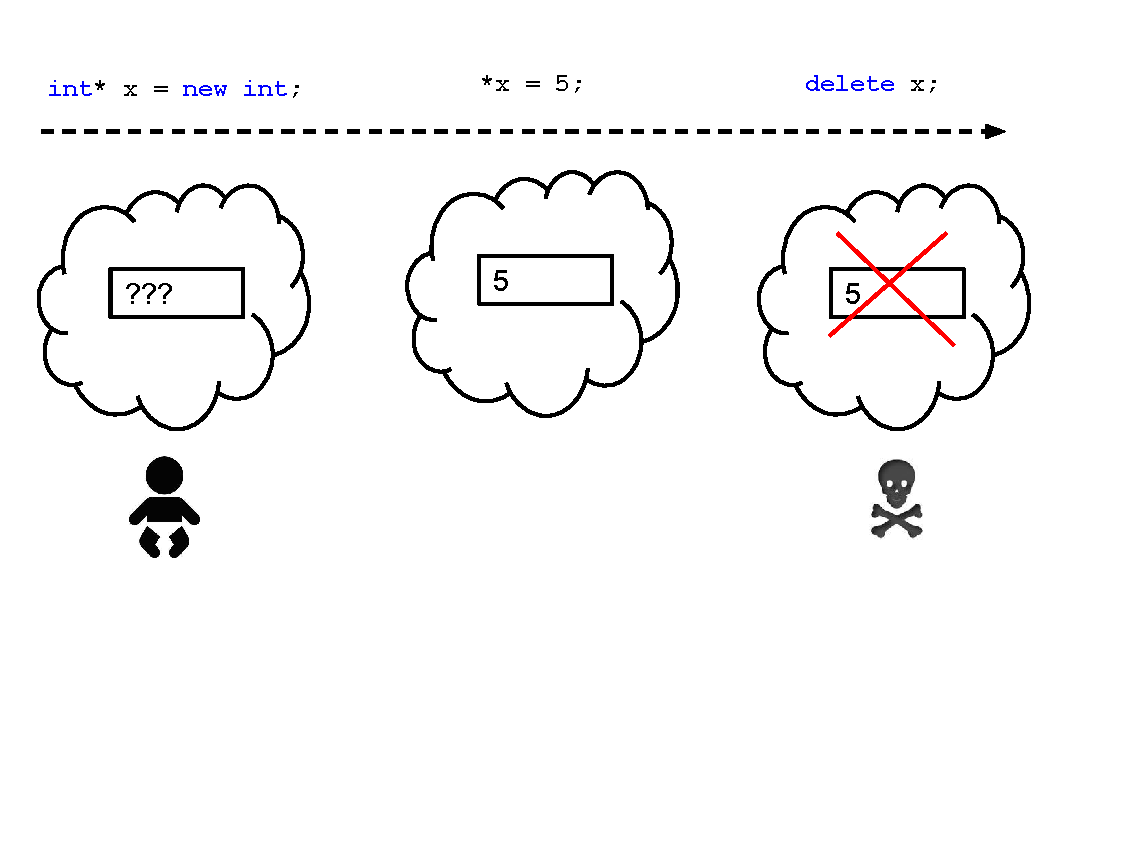
\includegraphics[width=12.5cm]{images/lc_heap}
\end{frame}



\begin{frame}
\centerline{Инициализация по време дефиниция}
\end{frame}



\begin{frame}[fragile]
\frametitle{Локална променлива}
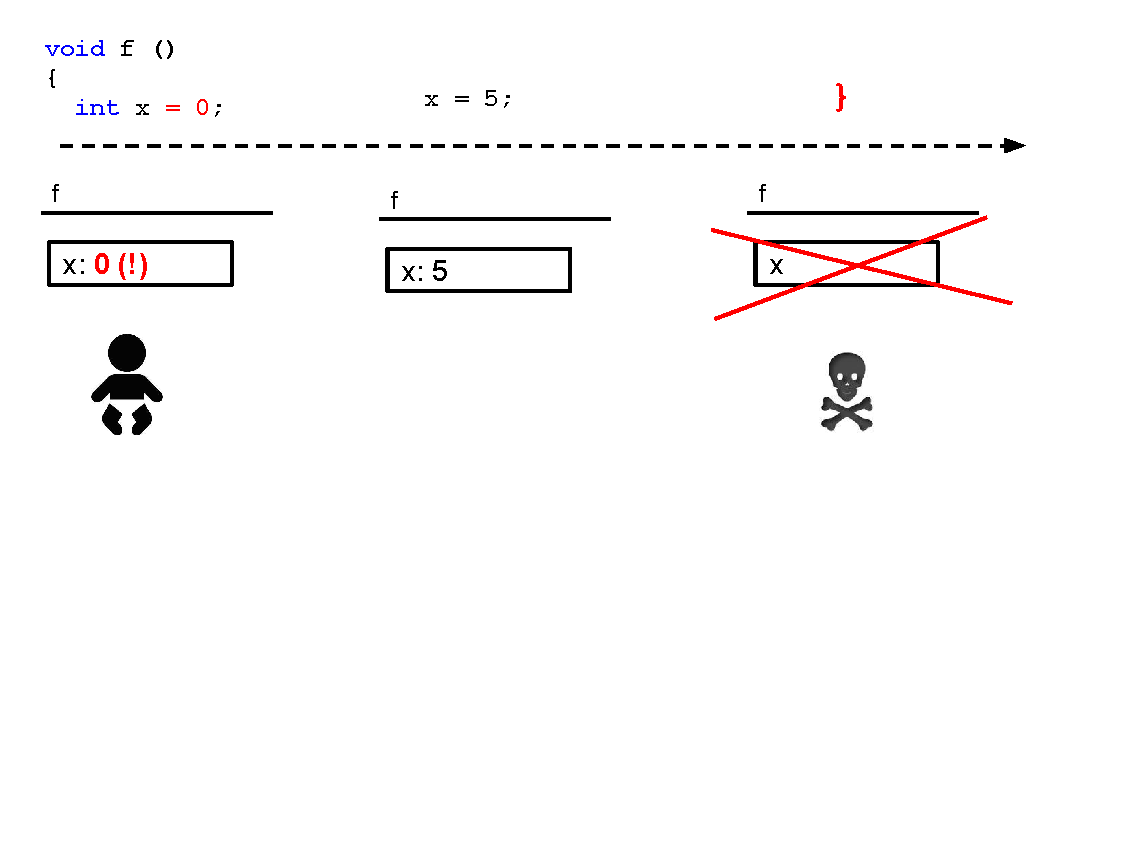
\includegraphics[width=12.5cm]{images/lc_var_cons}
\end{frame}


\begin{frame}[fragile]
\frametitle{Динамична памет}
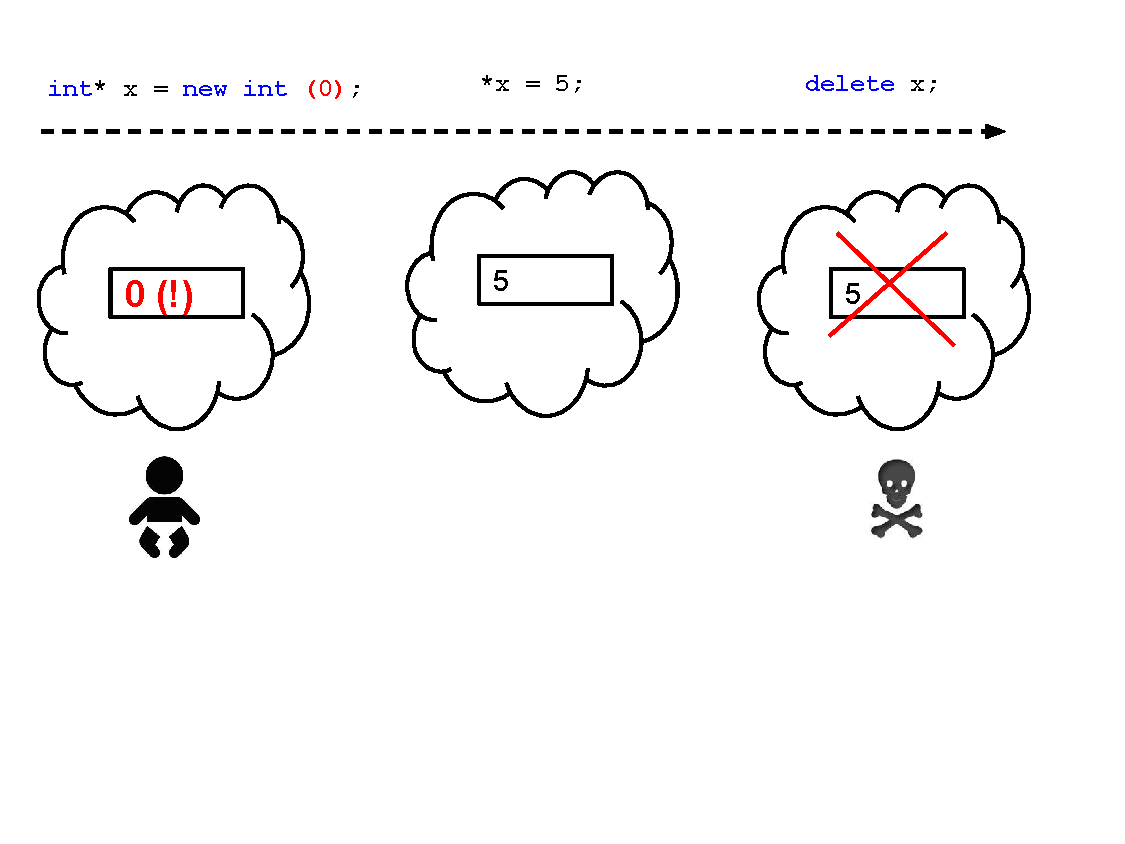
\includegraphics[width=12.5cm]{images/lc_heap_cons}
\end{frame}

\begin{frame}
\centerline{Конструктори}
\end{frame}

\begin{frame}[fragile]
\frametitle{С какви стойности е ``позволена инициализацията''}

\begin{itemize}
  \item ``Стандартни'', ``вградени'', ``прости'' типове

\begin{flushleft}
\relscale{0.75}
\begin{lstlisting}
double x = 1.2; // <=> double x (1.2);
double y = 1;
double z = 'q';
\end{lstlisting}  
\end{flushleft}


\end{itemize}

\end{frame}


\begin{frame}[fragile]
\frametitle{Потребителски дефинирани типове (пример: CharSet)}

\begin{itemize}
  \item Инициализация с низ (char*)

\begin{flushleft}
\relscale{0.75}
\begin{lstlisting}
CharSet s1 = "hello";
\end{lstlisting}  
\end{flushleft}
\pause
  \item Инициализация с буква (char)

\begin{flushleft}
\relscale{0.75}
\begin{lstlisting}
CharSet s2 = 'b';
\end{lstlisting}  
\end{flushleft}
\pause

  \item Инициализация с число

\begin{flushleft}
\relscale{0.75}
\begin{lstlisting}
CharSet s3 = 5;
\end{lstlisting}  
\end{flushleft}


\end{itemize}

\end{frame}

\begin{frame}[fragile]
\frametitle{Конструктор (от буква)}


\begin{flushleft}
\relscale{0.75}
\begin{lstlisting}
class CharSet
{
  //...

  void init ()
  { //CharSet* this
    for (int i =0; i < 26; i++)
      this->contents[i] = false;
  }

  //initialize with a single character
  CharSet (char c)
  {
    init ();
    this->contents[c-'a'] = true;
  }
};
\end{lstlisting}  
\end{flushleft}
\end{frame}


\begin{frame}[fragile]
\frametitle{Конструктор (от низ)}


\begin{flushleft}
\relscale{0.75}
\begin{lstlisting}
class CharSet
{
  //...

  CharSet (char *s)
  {
    init ();
    for (int i = 0; i < strlen(s); i++)
    {
      this->contents[s[i]-'a'] = true;
    }   
  }
};
\end{lstlisting}  
\end{flushleft}
\end{frame}


\begin{frame}
\centerline{Конструктор по подразбиране}
\end{frame}


\begin{frame}[fragile]
\frametitle{Без инициализация}


\begin{flushleft}
\relscale{0.75}
\begin{lstlisting}
CharSet s1;

//s1.init();
s1.print (); //NOT OK!!!

\end{lstlisting}  
\end{flushleft}
\end{frame}

\begin{frame}[fragile]
\frametitle{Задължителна (по подразбиране) инициализация}


\begin{flushleft}
\relscale{0.75}
\begin{lstlisting}
class CharSet
{
  //...
  CharSet ()
  {
    init ();
  }
};
int main ()
{
  CharSet s1;

  //s1.print();
  s1.print (); //OK!

}
\end{lstlisting}  
\end{flushleft}
\end{frame}


\begin{frame}
\centerline{Други ``автоматични'' конструктори}
\end{frame}


\begin{frame}[fragile]
\frametitle{``Вградени'' конструктори}

\begin{itemize}
  \item Инициализация с друг обект от същия тип 
\end{itemize}

\begin{flushleft}
\relscale{0.75}
\begin{lstlisting}

  CharSet s1 = "hello";
  CharSet s2 = s1; 

  s2.print();

\end{lstlisting}  
\end{flushleft}

\end{frame}

\begin{frame}
\centerline{Благодаря за вниманието!}
\end{frame}

\end{document}



\begin{columns}[t]
  \begin{column}{0.55\textwidth}

  \end{column}
  \begin{column}{0.45\textwidth}

  \end{column}
\end{columns}
